\subsection{SPAN Connectivity Model}

The protocol runs over an ad-hoc network,
where each node is a smartphone
and the nodes connect wirelessly to each other.
In the simulation,
we modelled this underlying infrastructure using a dynamic random graph.

The most commonly studied model of random graphs is the Erdős--Rényi model.
Given parameters $n$ and $p$,
the model generates a graph with $n$ vertices
and each edge is added to the graph independently with probability $p$~\cite{bollobas_2001}.
This model, however,
has no information about node positions,
which makes it a poor representative of ad-hoc networks~\cite{Hekmat2006}.

Instead,
we will use random geometric graphs as our connectivity model.
Given parameters $n$ and $r$,
the model randomly chooses $n$ points in the unit square $[0, 1]^2$,
uniformly and independently,
and adds an edge between each points which are at a distance $r$ from each other.
Random geometric graphs
have been proposed as accurate models for ad-hoc networks~\cite{Kenniche2010,Hekmat2006}.

Nodes which are close to the borders of the unit square
are affected by the so-called ``border effect'':
if the distance of a node is smaller than $r$
from any of the borders,
then part of the ``area of coverage'' for this node
(that is,
the area which may contain adjacent vertices)
lies outside of the unit square.
This effectively truncates the degree of that node,
because no nodes are generated outside the unit square.
For smaller values of $r$ this effect is less pronounced,
because less nodes are affected.

In order to avoid the border effect,
we will use toroidal distances instead~\cite{Kenniche2010,Hekmat2006}.
The nodes will be placed on the unit torus $[0, 1)^2$
and distances will be measured according to a toroidal metric.
So,
for example,
for $r = 0.1$,
the nodes at $(0.01, 0.01)$ and $(0.99, 0.99)$ are adjacent in this metric.

We will denote
the toroidal random geometric graph model with parameters $n$ and $r$
by $T(n, r)$.

We want to model the underlying infrastructure to be dynamic,
to represent the fact that nodes move around in the world.
That is,
we will have a sequence $G_0, G_1, \dots$ of graphs over the same set of nodes,
which represent the evolution of the network.

Using the toroidal has the benefit that
if the nodes move around randomly, but independently,
then each resulting graph is still a geometric graph.
More precisely,

\begin{proposition}
	Let $G_0 \in T(n, r)$ be a random graph.
	For each $i \in \mathbb N$,
	define $G_{i+1}$ by translating each vertex $v \in V(G_i)$
	by a random translation vector $u_v$,
	chosen independently according to some distribution,
	and connecting vertices which are within a distance of $r$ of each other.
	Then, for each $i$,
	the graph $G_i$ is a random geometric graph distributed according to $T(n, r)$.
\end{proposition}

Note that each $G_i$ will be distributed according to $T(n, r)$,
regardless of the distribution of the translation vectors $u_v$
(as long as each translation vector is chosen independently,
and irrespective of the vector $v$).

% TODO: Proof?

However,
there is nothing cohesive in the literature about using several different
translation parameters at once.
We will use a simplified version of the dynamic model of~\cite{Diaz2008}.
Fixed a parameter $s$,
$G_{i+1}$ is generated from $G_i$
by translating each vertex by a vector with norm $s$,
chosen uniformly among all $s$-normed vectors in $\mathbb R^2$.

% TODO: Picture?

\subsection{Visualizing the Interplay between Local and Semi-Global Chains}
Due to the SPANchain module existing for less than a quarter of a year, it
lacks a complete set of visualization tools for analyzing the
behavior of semi-global blockchains over SPANs. Partly, this is due to
our module being the first to accommodate forking as a feature rather than
a bug; the only degree to which forking is well-understood in the literature
is how one can best prevent it from happening. Though furthering our work
will require rigorous measures of semi-global blockchain formation and
diversity, we offer the following toy case as a proof of concept that the persistence of
semi-global chains in the network (i.e. the degree to which a non-trivial
global blockchain failes to exist) preserve information as to how the SPAN
topology has changed over time.

The top of Figure \ref{fig:old_town_road} shows a connected SPAN which maintains
its initial state long enough for ten blocks to form and propagate. The SPAN
then partitions into two connected components, remains in this state long enough for
ten more blocks to form and propagate, and finally reverts to its original state.
The simulation randomly grants and deterministically propagates ten more blocks before
terminating.

The bottom of Figure \ref{fig:old_town_road} shows the local blockchain held by a
specific node in the described SPAN. The local chain recognizes all blocks indices
zero through nine, as all problem formulations and blocks from all other nodes
reached the node in question. However, this node does not recognize all of blocks ten
through 19, as some of these were discovered by nodes in the other partition during the
period of disconnection. By the time the two partitions joined back together, we see two
branches in the local chain competing for status as global chain; one of these, which
begins with the edge from node zero to node 21, represents the continuation of what had
been the longest chain in the other partition. As half the nodes in the network recognize
it as the longest chain, leaves on this chain become parent references for roughly half
of the problem proposals created in the network. Though the branch which corresponds to
the global chain in what had been the node's own partition continues to grow, it is
actively competing with the continuation of the other partition's leading chain. This
long-term coexistence of these two branches is strictly an artifact of the network's
partition and reunification, and the lengths of the branches correspond to the duration
of this separation.

\begin{figure}
	\centering
	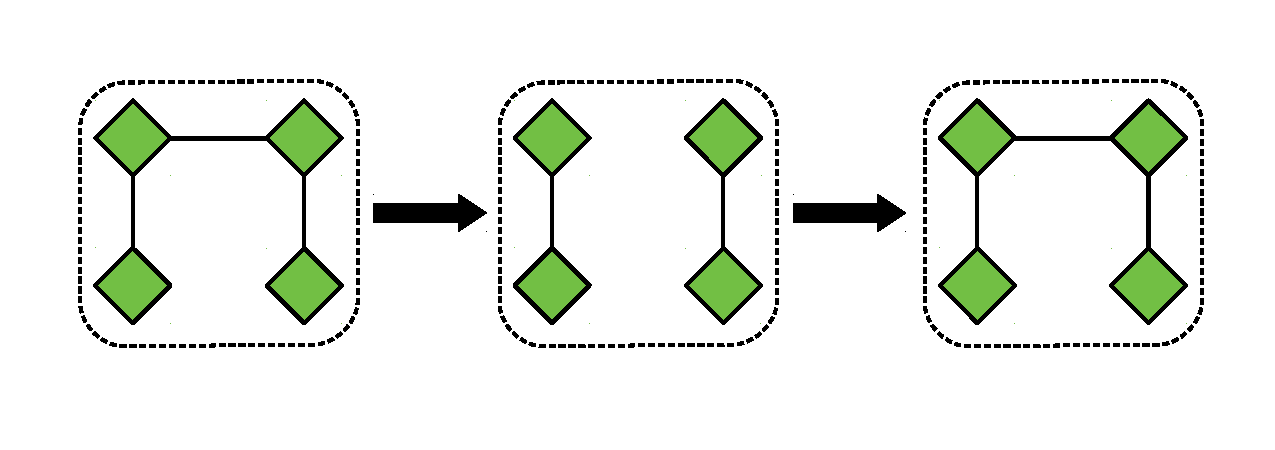
\includegraphics[width=\columnwidth]{horseshoe.pdf}
	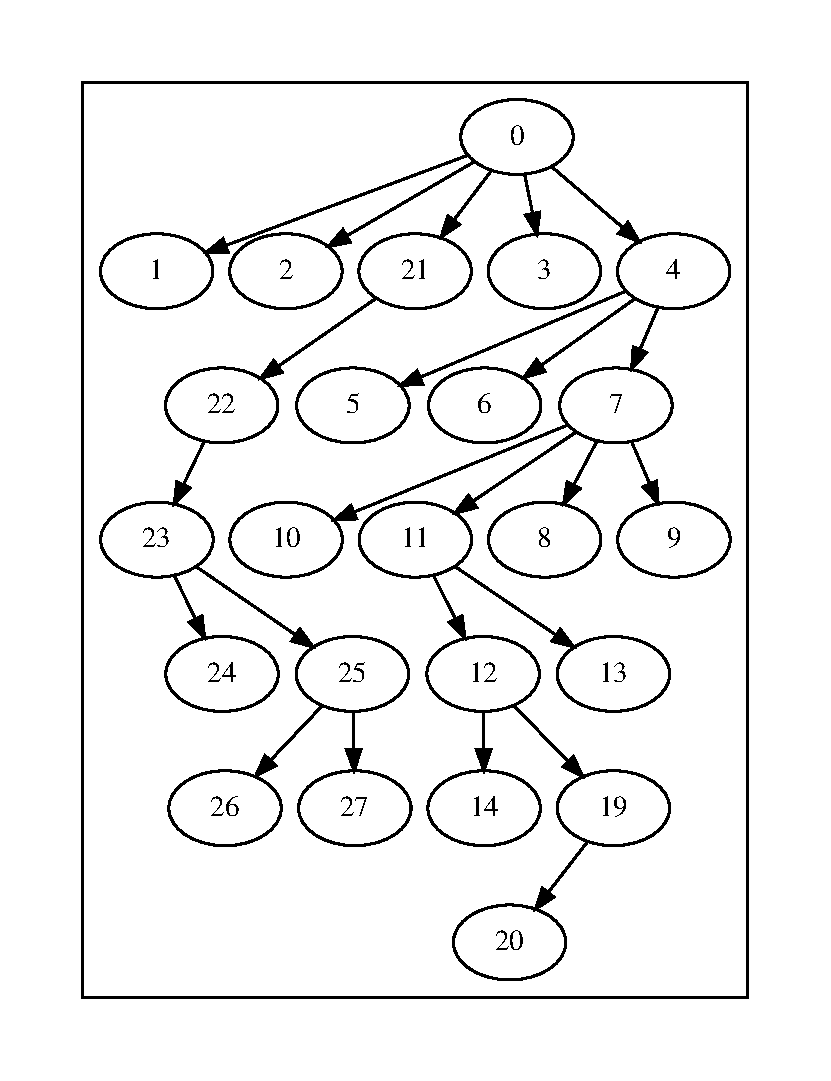
\includegraphics[width=\columnwidth]{horseshoe_0.pdf}
	\caption{A proof-of-concept SPAN-distribted blockchain simulated in SPANchain.
		The simulation is performed in the script \texttt{horseshoe\_partition.py},
		visualization of the output is performed using \texttt{make\_figures.sh}.}
	\label{fig:old_town_road}
\end{figure}
